\section{Timer and Interrupts}

\subsection{Modulo Counter}

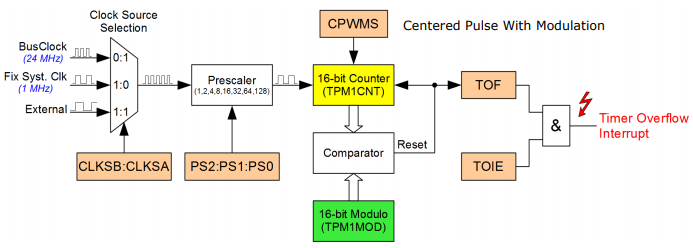
\includegraphics[width=0.5\textwidth]{timer-overview.png}

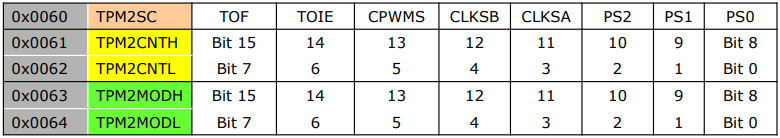
\includegraphics[width=0.5\textwidth]{timer-2-control-registers.png}

\subsection{Modulo Frequency}

$\mathbf{T_{TOF} = (MOD + 1) \cdot PS / f_{Clk}}$
\newline
\begin{itemize}
    \item{$\mathbf{T_{TOF}}$: Time between two Timer-Overflow events}
    \item{$\mathbf{MOD}$: Value of the Modulo set}
    \item{$\mathbf{PS}$: Presacler value}
    \item{$\mathbf{f_{Clk}}$: frequency of the controller}
\end{itemize}

\textit{
    \newline
    To calculate the modulo, the frequency (Clock Source) needs to be selected
    and the prescaler needs to be defined. To calculate the Modulo value, following can
    be used. The Modulo is 2 Bytes, so it needs to be between \textbf{0 < MOD < 65536}
    \newline
}

$\mathbf{MOD = (\frac{T_{TOF} \cdot f_{Clk}}{PS}) - 1}$

\subsection{Timer Control Registers}

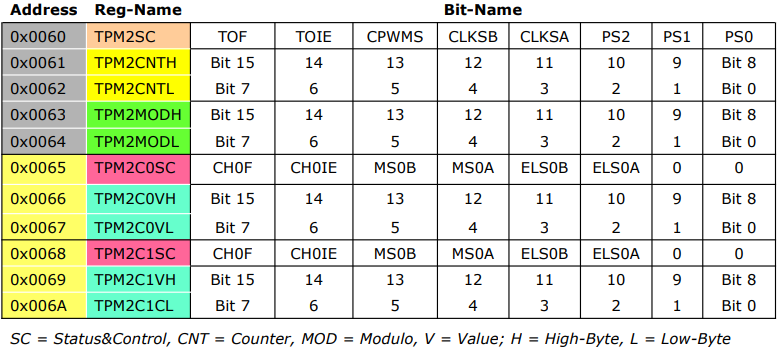
\includegraphics[width=0.5\textwidth]{timer-2-control-registers-channels.png}

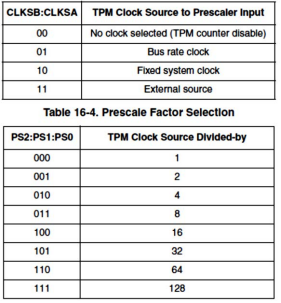
\includegraphics[width=0.5\textwidth]{timer-x-control-register-config.png}

\subsection{Polling and Interrupts}

\textit{
    A MC-System has to react instantly to events (internal or external)
    (e.g. measure value monitoring, serial communication).\newline
    The \textbf{instant of time} of these events is \textbf{not known in advance}. \newline
    There are two ways to react to those kind of events: \newline
}

\begin{itemize}
    \item{
        \textbf{Interrupt} = Exception handling \newline
        \textit{
            enables \textbf{realtime capable (+)} systems (depends on interrupt
            \textbf{latency}). \textbf{Fast reaction time} through automatic reaction
            to events and interrupt of the program to execute an
            Interrupt-Service-Routine (ISR). \newline
            Needs substancial effort for \textbf{state backup (-)}, because the instant of
            the program interruption is unknown.
        }
    }
    \item {
        \textbf{Polling} = cyclic requesting \newline
        \textit{
            \textbf{Shorter} program \textbf{interruption (+)}. Since the instant of time is
            known during programming, the state can be backed up more efficiently. \newline
            \textbf{esier to understand / debug (+)} \newline
            \textbf{Waste of caclulation time (-)} if events occure rarely
        }
    }
\end{itemize}

\textit{
    \newline
    Each MCU holds an Interrupt-Logic to realise real-time systems.
}

\subsection{Interrupt execution}

\begin{enumerate}
    \item{Interrupt called}
    \item{Save current state onto stack}
    \item{Call function}
    \item{By Programming - clear interrupt flag}
    \item{go back to code}
    \item{load saved state from stack}
    \item{keep running where stop before interrupt}
\end{enumerate}

\subsection{Save Interrupt State}

\begin{wrapfigure}{l}{0.3\textwidth}
    \centering
    \hspace{-20pt}
    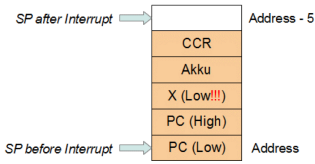
\includegraphics[width=0.3\textwidth]{stack-interrupt-state.png}
    \hspace{-50pt}
\end{wrapfigure}

\textit{
    On entrance to an ISR the CPU-State is backed up automatically to the
    Stack.
    \newline
    \newline
}

\textit{
    Note: The \textbf{H-Register} must be saved „manually“ on the HCS08 (only
    with Assembler)
}

\subsection{Difference ISR and Subroutines}

\textit{ISR = Interrupt Service Routine / Interrupt Subroutine}

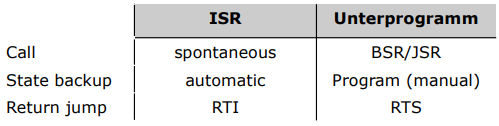
\includegraphics[width=0.5\textwidth]{isr-subroutine-difference.png}

\subsection{Interrupt Sources Priority}

\textit{
    In the MC9S08JM60 there are 29 Interrupt Sources, that are sorted by
    priority in the Interruptvector-Table
}

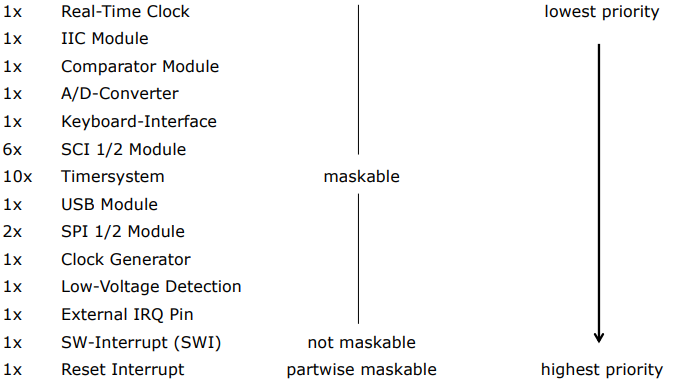
\includegraphics[width=0.5\textwidth]{interrupt-priority-list.png}

\textit{
    By default the HCS08 does \textbf{not support nested
    Interrupts}, because the I-Flag gets set on an entrance
    into an ISR. \newline
    If there are more Interrupt demands, the ISR with the
    highest priority (lowest vector number) is called first
}

\subsection{Interrupt Counter}

\textit{
    Setting the Interrupt Counter will set it always to 0.\newline
    Reading one of the Counter 8 Bit, the other one will be saved to a
    shadow register until read from.
}

\subsection{Interrupt Vectortable}

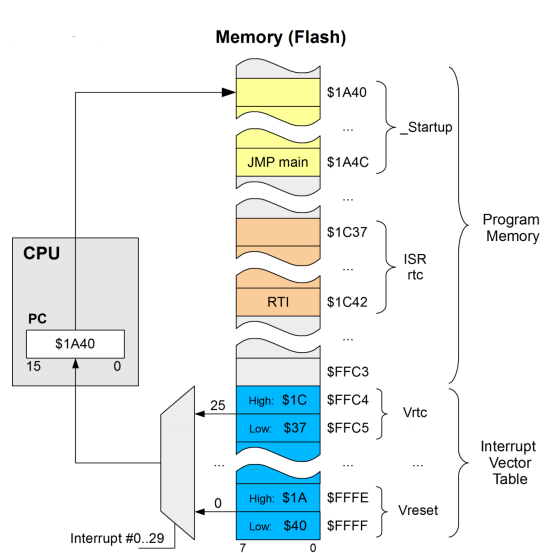
\includegraphics[width=0.5\textwidth]{interrupt-vector-table.png}

\begin{lstlisting}
// Extract out of .prm File
VECTOR ADDRESS 0xFFC4 ISR_RTI // RTC
VECTOR ADDRESS 0xFFC6 errISR_IIC // IIC
VECTOR ADDRESS 0xFFC8 errISR_ACMP // ACMP
VECTOR ADDRESS 0xFFCA errISR_ADC // ADC Conversion
...
VECTOR ADDRESS 0xFFDA motorBoosterISR // TPM2 overflow
VECTOR ADDRESS 0xFFDC errISR_TPM2CH1 // TPM2 channel 1
VECTOR ADDRESS 0xFFDE errISR_TPM2CH0 // TPM2 channel 0
VECTOR ADDRESS 0xFFE0 errISR_TPM2O // TPM1 overflow
VECTOR ADDRESS 0xFFE2 errISR_TPM1CH5 // TPM1 channel 5
VECTOR ADDRESS 0xFFE4 errISR_TPM1CH4 // TPM1 channel 4
VECTOR ADDRESS 0xFFE6 errISR_TPM1CH3 // TPM1 channel 3
VECTOR ADDRESS 0xFFE8 errISR_TPM1CH2 // TPM1 channel 2
VECTOR ADDRESS 0xFFEA errISR_TPM1CH1 // TPM1 channel 1
VECTOR ADDRESS 0xFFEC ifrFrontISR // TPM1 channel 0
\end{lstlisting}

\subsection{Interrupt-Release Logic}

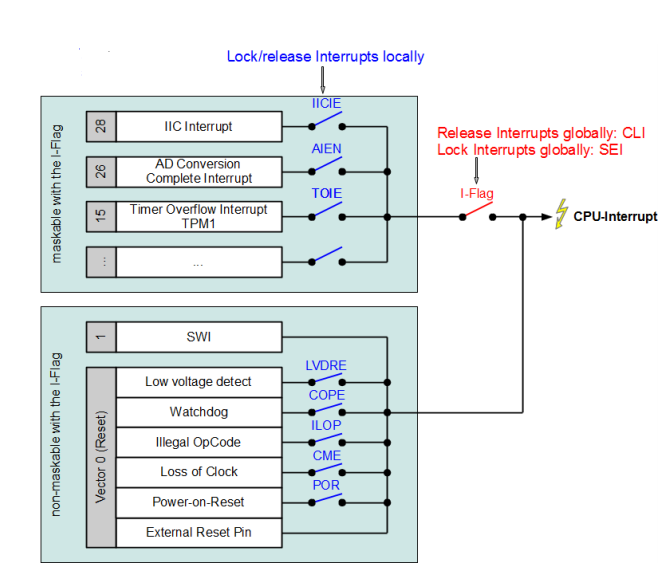
\includegraphics[width=0.5\textwidth]{interrupt-release-logic.png}

\subsection{Programming of Interrupts}

\textit{Following is important for programming interrupts:}

\begin{itemize}
    \item{
        \textit{
            Define \textbf{Interruptvectors}; at the place of the Interruptvector
            has to be the start address of the ISR (in CW definition in .prm file)
        }
    }
    \item{
        \textit{
            Define and initialise \textbf{Stack}
        }
    }
    \item{
        \textit{
            \textbf{Delete} the Interrupt-\textbf{Flags before} you release them, so that the Interrupt
            does not get fired right away.
        }
    }
    \item{
        \textit{
            Programming of ISR; CPU-State gets backed up automatically (H-Register
            only through C-Compiler)
        }
    }
    \item{
        \textit{
            \textbf{Delete} the Interrupt-\textbf{Flag} in the ISR
        }
    }
    \item{
        \textit{
            End the ISR with \textbf{RTI} (is done automatically on usage of C-Compiler)
        }
    }
    \item{
        Release Interrupts globally (\textbf{CLI}) in the main program
        (typically after initialisation part)
    }
\end{itemize}

\begin{lstlisting}
interrupt void myTofISR(void)
{
    // myTofISR function needs to be mapped
    // in the vectortable -> parameterfile (.prm).
    //reset the interrupt flag
    TPM1SC_TOF = 0;

    //run logic
}
void initTimer(void)
{
    //set module to 25780 / 0x64B4
    TPM1MODH = 0x64;
    TPM1MODL = 0xB4;
    //TPM1MOD = 25780;
    //Clock set to 1 MHz
    TPM1SC_CLKSA = 0;
    TPM1SC_CLKSB = 1;

    //define Prescaler to 128
    TPM1SC_PS0 = 1;
    TPM1SC_PS1 = 1;
    TPM1SC_PS2 = 1;

    // reset counter
    TPM1CNT = 0

    // enable timer Overflow Interrupt
    // this should be the last action
    TPM1SC_TOIE = 1;
    // Reset the Timer Overflow Interrupt
    TPM1SC_TOF = 0;
}
void main(void)
{
    initTimer();
    //enable interrupts
    EnableInterrupts;
}
\end{lstlisting}
